\section{UES - Join Ordering with Simple Upper Bound}
\label{sec:UES}

In contrast to state-of-the-art approaches (see Section~\ref{sec:RealtedWork}), our UES concept~\cite{hertzschuch-21-ues} follows a completely different idea to determine good join orderings for SPJ queries: instead of trying to obtain precise estimates for join cardinalities, it calculates theoretical upper bounds of the sizes of intermediate result sets and uses these bounds in a heuristic join enumeration algorithm. 
This concept is based on the insight that the duration of query workloads is often dominated by the runtime of very few queries that take an exceptionally long amount of time. 
Meanwhile, most queries in a typical workload can be answered rather quickly. 
This phenomena is referred to as \emph{tail latency}.
Thus, a novel query optimization strategy should focus on improving these long-running queries, instead of speeding up queries that are already fast. 
However, this can usually not be achieved by improving the runtime in the average case, since new outliers can become part of the tail latencies. 
In contrast, a correct theoretical upper bound can never be wrong in the sense that the true cardinalities exceed the bound. 
By feeding these worst-case estimates to the join enumeration algorithm, it will probably choose a join order that is too pessimistic in the sense that another join order could have provided a faster runtime. 
But it will never choose a join order that is too optimistic, i.e. a plan that only works if the intermediate cardinalities are indeed small and takes a much longer time to execute if this hope is not met. Following this general philosophy of focusing on the long running queries, it is acceptable if very fast queries get slightly slower, as long as the tail latencies are removed. In the following, we sketch both the upper bounds for join cardinalities, as well as the heuristic join enumeration algorithm of UES.

Our UES upper bounds of join intermediate cardinalities are estimated via most frequent value statistics on the join columns. In fact, the only metadata necessary to calculate upper bounds with UES are the frequencies of the most common values of the join attributes and the total number of (filtered) tuples per base table. These statistics are then combined with a number of pessimistic assumptions regarding the distribution and correlation of the attribute values.
For brevity the calculation is only summarized here, since the final formula is already presented and justified in~\cite{hertzschuch-21-ues}.
To estimate the size of a join $R.x \bowtie S.y$ on (filtered) base tables $R$ and $S$ while only using the most frequent values for $R.x$ and $S.y$, a first pessimistic assumption is used: the attributes are \emph{assumed} to be uniformly distributed, with the maximum value frequency (MF) therefore also being the only frequency shared by all values. 
Based on these frequencies and the total number of tuples per (filtered) relation ($|\sigma(R.x)|, |\sigma(S.y)|$), the minimum number of distinct values per attribute can be estimated as $|\sigma(R)| / MF(R.x)$ for $R$ and likewise for $S$.
To combine these per-table values into an estimate for their join result, a second pessimistic assumption is used: the attribute values are \emph{assumed} to overlap perfectly, i.e. each value in $R.x$ has a matching join partner in $S.y$ and vice-versa. 
This leads to $MF(R.x) \cdot MF(S.y)$ many outgoing tuples per value combination due to the uniformity assumption. 
Since there are at most $min(|\sigma(R.x)| / MF(R.x), |\sigma(S.y)| / MF(S.y))$ many such combinations, the upper bound can be calculated as
$$upper(|\sigma(R) \bowtie \sigma(S)|) := min\Bigl(\frac{|\sigma(R)|}{MF(R.x)}, \frac{|\sigma(S)|}{MF(S.y)}\Bigr) \cdot MF(R.x) \cdot MF(S.y)$$

\begin{figure}[t]
    \centering
    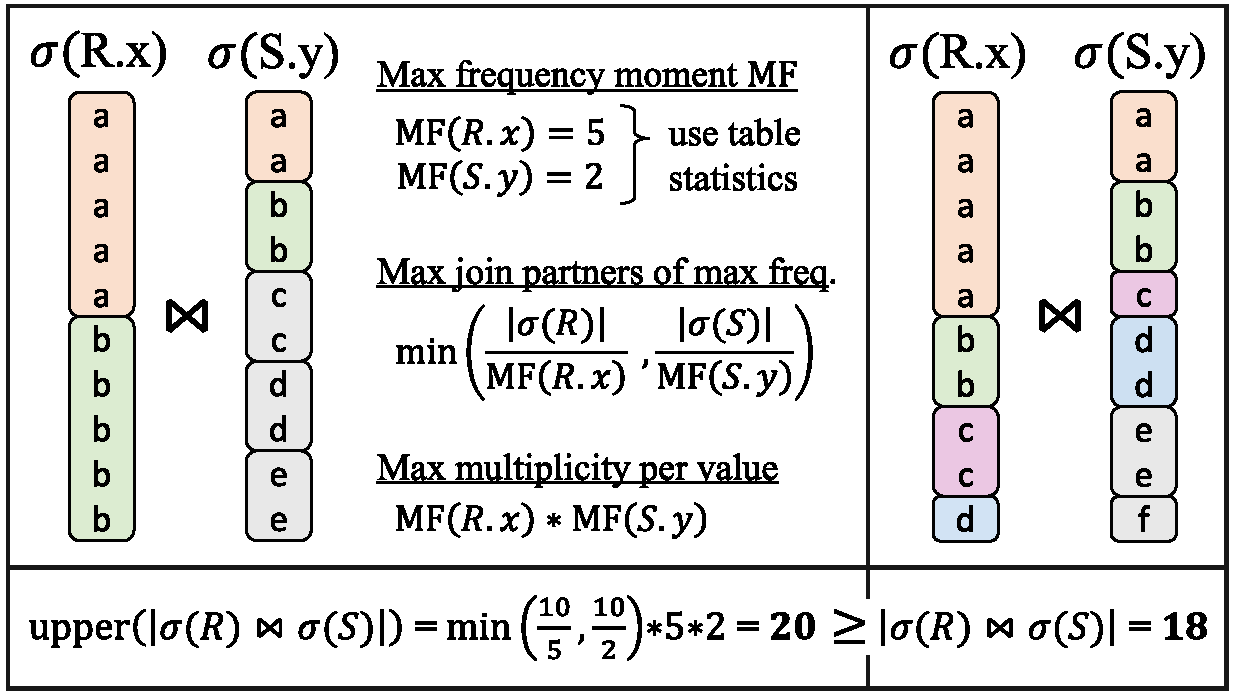
\includegraphics[width=0.7\linewidth]{figures/upperBoundExplV6_.pdf}
    \caption{Illustration of the UES upper bound (taken from \cite{hertzschuch-21-ues}).}
    \label{fig:upperBoundExpl}
\end{figure}

Fig.~\ref{fig:upperBoundExpl} illustrates our UES upper bound concept, using an example. 
The left-hand side depicts the worst-case -- used to derive the upper bound -- constrained by the table statistics, while the right-hand side depicts the actual join.
Note that $R$ and $S$ do not need to be base tables. 
Instead they can be the result of some other join just as well. 
For example, without loss of generality, we can assume that $R = R_1 \bowtie_{R_1.x = R_2.y} R_2$. 
In this case, $|\sigma(R)| = upper(|R_1 \bowtie R_2|)$ and $MF(R.x) = MF(R_1.x) \cdot MF(R_2.y)$. 
This enables the calculation of upper bounds for any join in a recursive manner. 
One central downside of this approach is the propagation of errors, in this case of overestimated result sizes. 
Since the estimation of an $n$-way join requires estimates of $n-1$ smaller joins building on top of each other, estimates grow larger and larger as already shown in Fig.~\ref{fig:UESOverestimationJOB}.
%This puts special emphasis on the importance of tight upper bounds. 

Based on this upper bound for join cardinalities, the join order in UES is obtained using a heuristic algorithm~\cite{hertzschuch-21-ues}.
The UES join enumeration algorithm tries to choose each join such that the sizes of intermediate results are minimized in each step. 
To make this choice, the upper bounds of candidate joins are calculated and the join with smallest bound is executed. 
However, this process is only applied to n:m joins. 
Primary key/foreign key joins (P/K joins) are greedily included as soon as possible. 
This strategy is justified by a central property of P/K joins: When the foreign key partner is already present in the intermediate result, joining the primary key table may only reduce but never expand the size of the intermediate result. In this sense, P/K joins act as special filters. 
To facilitate this filtering property even further, a P/K join can be executed as a subquery: suppose an (intermediate) table $\Tilde{T}$ should be joined with a foreign key table $T_{FK}$, which in turn has to be joined with a Primary Key table $T_{PK}$. 
The canonical way of executing this join would be $(\Tilde{T} \bowtie T_{FK}) \bowtie T_{PK}$. The n:m join $\Tilde{T} \bowtie T_{FK}$ would most likely (i.e. following the pessimistic assumption) increase the size of the intermediate result. 
Afterwards, joining $T_{PK}$ could potentially reduce the size of the intermediate result again. 
If such a reduction is guaranteed, executing $T' := T_{FK} \bowtie T_{PK}$ first and afterwards $\Tilde{T} \bowtie T'$ would minimize work for the second join. Thus, when choosing the next n:m join to execute, UES tries to pre-filter the join partners via P/K joins. 
If this does not guarantee a smaller intermediate result, the Primary Key partner will be joined after the n:m join has been executed. To some extent, this strategy resembles the well-known pushdown of filter predicates.

To better illustrate the concept of P/K filters, consider part of query 8d of the JOB: \sql{SELECT * FROM cast\_info ci, company\_name cn, movie\_companies mc WHERE cn.country\_code = '[us]' AND mc.company\_id = cn.id AND ci.movie\_id = mc.movie\_id}. Overall, this query fragment produces about 59 million result tuples. It contains one P/K join between \sql{movie\_companies} and \sql{company\_name} and one n:m join between \sql{cast\_name} and \sql{movie\_companies}. In this case, the P/K join $mc \bowtie cn$ reduces the cardinality of \sql{movie\_companies} from about 5 million to 2 million. This essentially halves the work for the following n:m join between \sql{cast\_name} and \sql{movie\_companies}, since \sql{company\_name} ``filtered'' its P/K partner.
